\documentclass[10pt,b5paper, twocolumn]{ltjsarticle}
\usepackage[paper=b5j, bmargin=100pt]{geometry}
\usepackage{luatexja}
\usepackage[utf8]{inputenc}
\usepackage[backend=biber, style=numeric]{biblatex}
\addbibresource{references.bib}
\usepackage{amsmath}
\usepackage{amssymb}
\usepackage{mathtools}
\usepackage{leadsheets}
\makeatletter
\let\meterC\relax
\makeatother
\usepackage{musicography}
\usepackage{luatexja-ruby} 
\usepackage{wrapfig}
\usepackage{caption}
\usepackage{makecell}
\usepackage{dashrule}
\usepackage{graphicx}
\usepackage{adjustbox}
\usepackage[dvipsnames]{xcolor}
\graphicspath{ {./resources/} }
\usepackage{hyperref}
\usepackage{subcaption}
\usepackage{csquotes}
\usepackage[document]{ragged2e}

\setchords{
    major-seven = \textsuperscript{M7},
    major-nine = \textsuperscript{M9}
}

\renewcommand*\contentsname{目次}
\renewcommand{\figureautorefname}{図}
\renewcommand{\tableautorefname}{表}
\renewcommand{\subsectionautorefname}{節}
\setlength{\RaggedRightParindent}{\parindent}
\setlength{\abovecaptionskip}{0pt plus 3pt minus 2pt}
\RaggedRight
\pagenumbering{roman}
\addtocounter{page}{1}
\setcounter{tocdepth}{2}

\title{\huge{コードオタクが語る東方楽曲分析}  \vspace{3pt} \hrule \vspace{3pt} {\large{第四弾　U.N.オーエンの狂気と希望}}}
\author{{Metalloid.}}
\date{{2026-10}}

\newcommand{\wc}{\writechord}
\NewDocumentCommand{\sd}{}{\musDegree}
\definecolor{bgc}{RGB}{255, 245, 206}


\begin{document}
\maketitle

%{\huge{コードオタクが語る東方楽曲分析}}
%\vspace{3pt}
%\hrule
%\vspace{3pt}
%\rightline{\large{第三弾　風神少女から垣間見る\ruby{調}{キー}からの逸脱}}
%\vspace{12pt} \rightline{Metalloid.} \rightline{10/2025}

\tableofcontents

\vspace{12pt}
\hrule
\vspace{12pt}
\section{まえがき・テーマ}
どうも、Metalloid.です。ちょうど先月、歴史的なことに東方紅魔郷のリメイクが出たことで、現在改めて東方紅魔郷の楽曲が世間の注目を浴びていることでしょう。特に、新たな楽曲リメイクおよび作者コメントが出たことによって、原曲の解釈の仕方に対して更なるヒントが出たかと思います。\par
そういった中で今回はフランドールのテーマ「U.N.オーエンは彼女なのか？」を取り上げていこうと思います。当楽曲のリメイクについて、ZUN氏は以下のようにコメントしています。\cite{EoSDNC}
\begin{displayquote}
    \textelp{} 殆どの二次創作が、
狂気か可愛さを強調された曲になっているのですが、自分はこの
曲に悠久の時間と無念さを込めたつもりで、そこを強調しました。
しかしそこはNewClassic版！　２４年を経て、最後にほんの少し
だけ希望と未来へと動き出す感情を追加しましたよ！ 
\end{displayquote}
U.N.オーエンが「狂気の音楽」として語り継がれてきたことは今や間違いないでしょう。とはいえ、この曲を狂気の一点張りとして解釈してしまうのはあまりにも勿体無いと考えております。本稿では、当楽曲がそのように解釈されてきた理由を音楽的観点から分析した後、楽曲が孕む「希望」について迫っていこうと思います。そして最後に、これが「亡き王女の為のセプテット」と如何に関係しているのかについて短く議論していきます。\par
前回23号で寄稿した第三弾―「風神少女」の分析はかなり本格的な記事になっていましたが、今回は音楽経験が少ない方でもある程度楽しめるように議論を進めていこうと思います。\par
\vspace{10pt}
\begin{figure}[h]
    \centering
    
\includegraphics[width=0.3\linewidth]{qr.png} 
    \label{fig:qr}
    \caption*{音声コンテンツ}
\end{figure}
前回同様、本稿の譜例に対応する簡単な音声ファイルを準備しているので、是非ご活用ください～
\par
\section{本題}
\subsection{U.N.オーエンと「狂気」}
本稿では「U.N.オーエンは彼女なのか？」(2002)が「狂気の音楽」として位置付けられる音楽的な根拠を以下の三点と考え、これを順番に見ていきます。
\begin{itemize}
    \item イントロの不可解なリズムと不協和音
    \item Aメロのスケールアウトと無機能和声
    \item 遠隔調への転調
\end{itemize}
\subsubsection{イントロの不可解なリズムと不協和音}
U.N.オーエンの印象的なそのイントロでいきなり聴者を迎えるのは所謂変拍子です。いかにも感覚的に乗りにくいこの5/4拍子\footnote{5/4拍子は五拍子としても解釈できますが、「ミッションインポッシブル」のように拍の長さが変わる四拍子として捉えることが多いです\cite{oddTimeSignatures}。}についてですが、リズムを細かく見ていくとさらなる特徴があります。\autoref{fig:intro}で見えるように、各小節は不可解なシンセが高速で走る「前半」と、コードプレイの三連打がみられる「後半」に二分されています。特にこの後半の二拍が二拍三連符で刻まれるていることが聴者のリズム感覚を乱します。また、和音の移り変わりのペースもわずか（東方原曲にしては珍しく）二拍となるため、聴者に焦燥が与えられます。\par
\begin{figure}[h]
    \centering
    
\includegraphics[width=\linewidth]{intro.png}
    \caption{イントロ}
    \label{fig:intro}
\end{figure}
使われている和音を実際に見てみると、二小節目の二和音目に東方原曲ではもはや珍しいものが使われています。この\wc{Co/Eb} (\wc{iio})は不協和音の類で、強い不安定感を与えます。また、五小節目からちょっとした変化球が入りつつ、六小節目の二和音目でまた別の不協和音（\wc{Ao7}）(\wc{viio7})が顔を出します。これは譜例に見える\na 記号から見えるように、一部スケールから外れた音を含みます。
\begin{figure}[h]
    \centering
    \fcolorbox{black}{bgc}{
        \begin{minipage}{\linewidth}
        \textbf{スケール（音階）} \\ 
        音には\sh ・ \fl を含んで12種類の音があるが、一枚の絵画で全ての色を用いないように、音楽でも限られた七つの音のみを使って音楽を構成することがほとんど。この七つの音の集合をスケールと呼ぶ。U.N.オーエンで用いられるスケールは主にB\fl マイナーであり、それはB\fl~C~D\fl~E\fl~F~G\fl~A\fl から成る。
        \end{minipage}
    }
\end{figure}
\subsubsection{Aメロのスケールアウトと無機能和声}
イントロと並ぶくらい印象的なAメロの最大の特徴は、半分近くの音が音階から外れていることでしょう。\autoref{fig:verse}の譜例にわかりやすさのために音階外の音に色を付けたのが\autoref{fig:verseAccidentals}となります。\par
\begin{figure}[h]
    \centering
    
\includegraphics[width=\linewidth]{verse.png}
    \caption{Aメロ}
    \label{fig:verse}
\end{figure}
\begin{figure}[h]
    \centering
    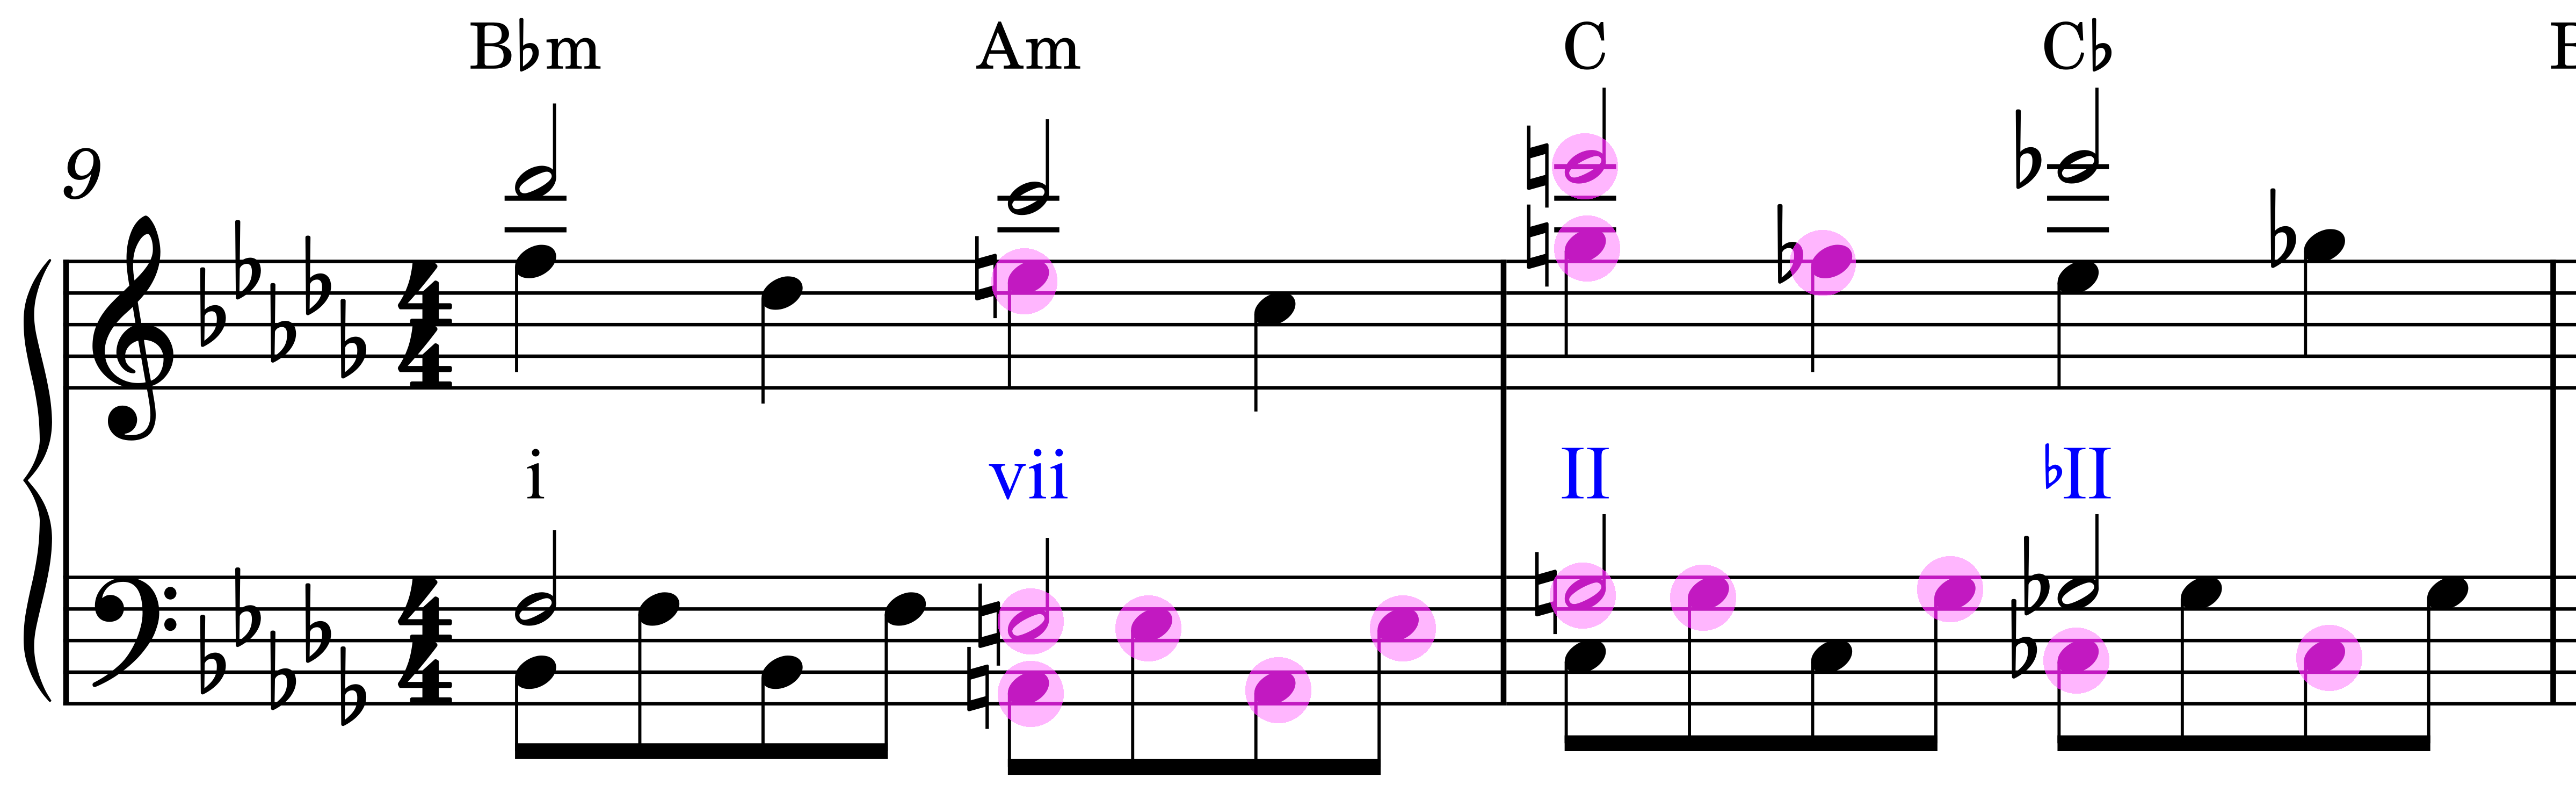
\includegraphics[width=\linewidth]{verseAccidentals.png}
    \caption{Aメロの音階外音}
    \label{fig:verseAccidentals}
\end{figure}
ストリングス、メロディー、ベースラインどれをとっても音階外音で詰められていて、聴者の調性感覚が乱されます。特にメロディーは音階外音を踏みながらエラティカルに上下する不可解なものとなっているので、これが「狂気」として解釈されることは自然な結果でしょう。\par
続けて和声に目を向けます。このAメロで音階外の音が多く出現することは和声に大きな影響を与えています。普通の曲では、コードは一般に「落ち着く」「不安定」「勢いづくり」のような役割（付録参照）を持ち、これらを順番に組み合わせることによって起承転結を構成します。ところがこのAメロのコード進行\wc{Bbm} \wc{Am} \wc{C} \wc{Cb}は調に存在しない和音がほとんど用いられているため、登場するコードはもはやそのような「役割」を持ちえません。異質な音の連続により唯単に偶発的に形成された和音が並列されていると捉えるべきでしょう。つまり、このAメロは「目的もなくランダムに徘徊する音および和音」で構成されている考えることができます。文字通り「狂」っていますね。
\subsubsection{遠隔調への転調}
U.N.オーエンのもう一つの驚異的な要素はサビ後のCメロでしょう。このCメロだけU.N.オーエンの主調から四半音上に転調しているのです。\autoref{fig:keyOverview}はその調関係を図示したものです\footnote{この図は五度圏といい、共通音が多い調同士が円上で接近して配置される図で、調の遠さ$\cong$転調を滑らかに済ませる難しさを図解できます。}。音楽的な繋がりが強固な三半音上下調への転調は東方原曲でも多いですが、足がかりの少なく飛びにくい四半音上下の転調はかなり珍しいもので、「変わっている」とも言えます。\par
\begin{figure}[h]
    \centering 
    
\includegraphics[width=\linewidth]{bridge.png} 
    \caption{Cメロ}
    \label{fig:bridge}
\end{figure}
\begin{figure}[h]
    \centering 
    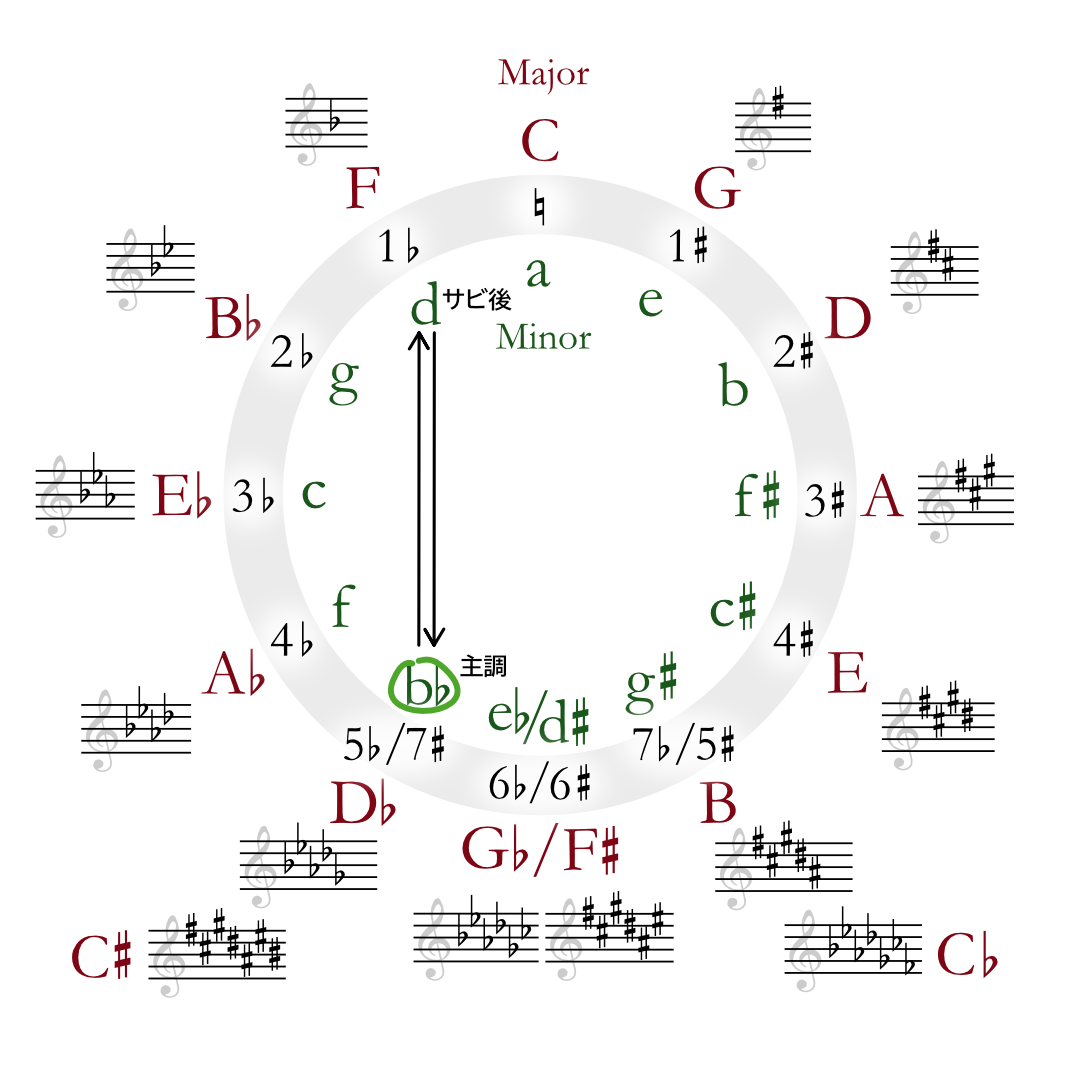
\includegraphics[width=\linewidth]{keyOverview.png} 
    \caption{転調鳥瞰図\cite{circleFifths}}
    \label{fig:keyOverview}
\end{figure}
転調オタクに向けて転調方法の詳細な分析も行ってみましょう。B\fl マイナーからDマイナーへの転調に用いられているのは\wc{Bbsus4}です。\wc{Bbsus4}は本来\wc{Bb}（或いは\wc{Bbm}）の和音を誘致するもので、その過程で\wc{Bbsus4}の構成音であるE\fl がD\na に下降してサスペンションが解決します。\wc{Bbsus4}と\wc{Dm}の連結をみていくと、E\fl の声部は確かにD\na に下降し解決しますが、それと同時に本来動かないはずのB\fl の声部が半音下降してA\na に落ちます。これによって、\wc{Bbsus4}から\wc{Bb}に解決する代わりに\wc{Dm}へと流れていくのです。\par
\begin{figure}[h]
    \centering 
    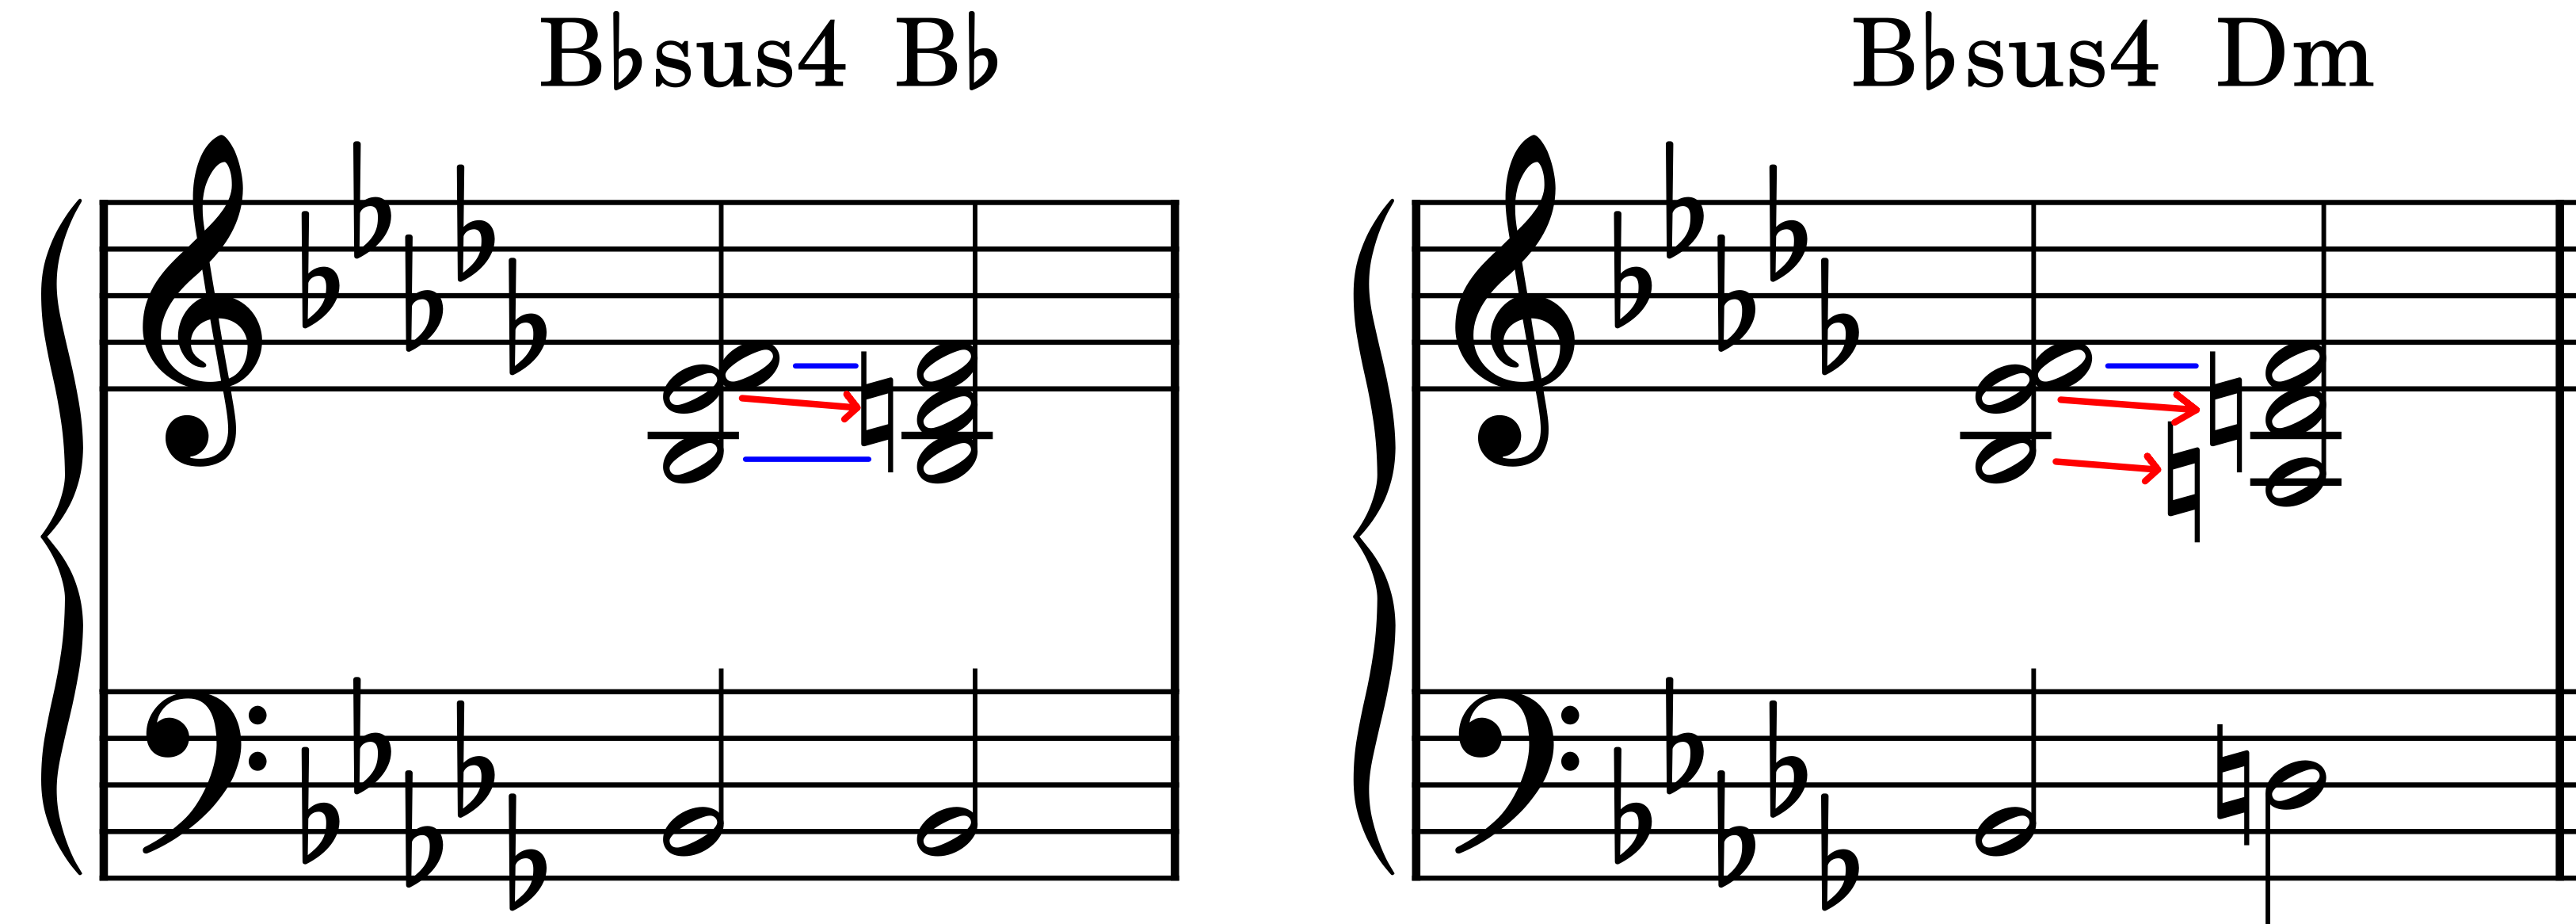
\includegraphics[width=\linewidth]{suspension.png} 
    \caption{\wc{Bbsus4}と\wc{Bb}および\wc{Dm}の連結のイメージの比較。青線は保続音、赤矢印は半音下降を示す。}
    \label{fig:suspension}
\end{figure}
続けて、DマイナーからB\fl マイナーへの戻り方を確認してみましょう。転調前の進行は\wc{Bb} \wc{C} \wc{C#o} \wc{C#+}\footnote{+はaugの略記。}(\wc{bVI} \wc{bVII} \wc{viio} \wc{VII+})となります。\wc{Bb}から\wc{C}は一般的な\wc{bVI} \wc{bVII}で、そこから和声短音階を用いることによりCをC\sh へ変化させ、\wc{C#o}を打ちます。ここまでは一般的なパターンですが、真に注目するべきはここからです：ポップスらしく\wc{C#o}をそのまま保続させるのではなく、最後に\wc{C#+}を打っています。ここで理解の鍵となるのはaug和音の長三度転回対称性です。\wc{C#+}は\wc{A+}や\wc{F+}と全く同じ構成音を持ちます。つまり、\wc{Dm}に対する\wc{V7}にあたる\wc{A7}を打つのと似たような発想で\wc{A+}($\cong$ \wc{C#+})を打っているという解釈が可能です。そして同時にそれは\wc{Bbm}に対する\wc{V+}にあたる\wc{F+}をも兼ねる、というのが転調のポイントとなります。

\subsection{U.N.オーエンの孕む「明るさ」} \label{sec:chorus}
これまでの分析ではU.N.オーエンが如何にも不可解な曲であるように思われてしまいますが、サビになるとこの曲は全く異なる毛色を見せます。これまでの不可解さが全く嘘であったかのように、サビはシンプルでわかりやすく、そして明るいといえるでしょう。\par
\begin{figure}[h]
    \centering
    
\includegraphics[width=\linewidth]{chorus.png}
    \caption{サビ}
    \label{fig:chorus}
\end{figure}
サビの「わかりやすさ」を生む要因はその最初のコード進行で、これは東方原曲で使いまわされている、ZUN氏デフォルトのコード進行（\wc{bVI} \wc{bVII} \wc{i}）から成ります。Aメロまでの「方向性の無さ」がここで一気に払拭され、再び前進するコード進行の中で聴者は方向感覚を取り戻すことができます。この楽曲構成法は「ハルトマンの妖怪少女」でも用いられております。\par 
\begin{figure}[h]
    \centering
    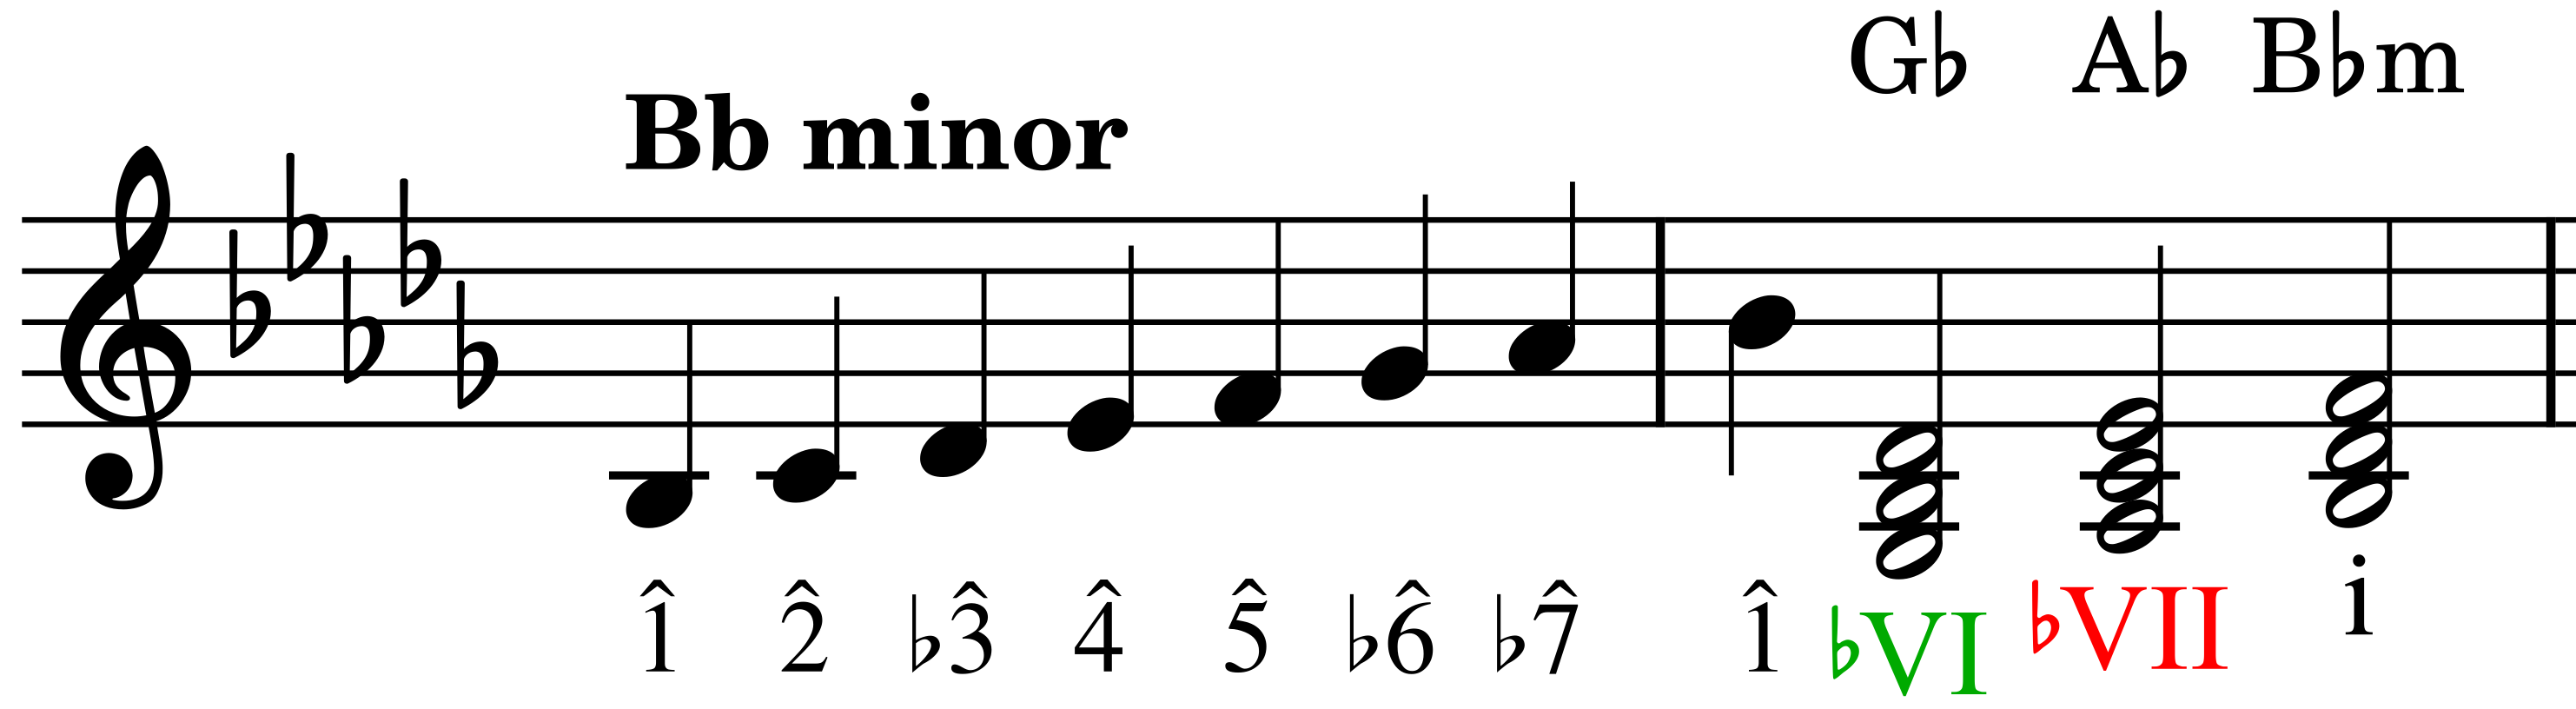
\includegraphics[width=\linewidth]{minorScale.png}
    \caption{自然短音階}
    \label{fig:minorScale}
    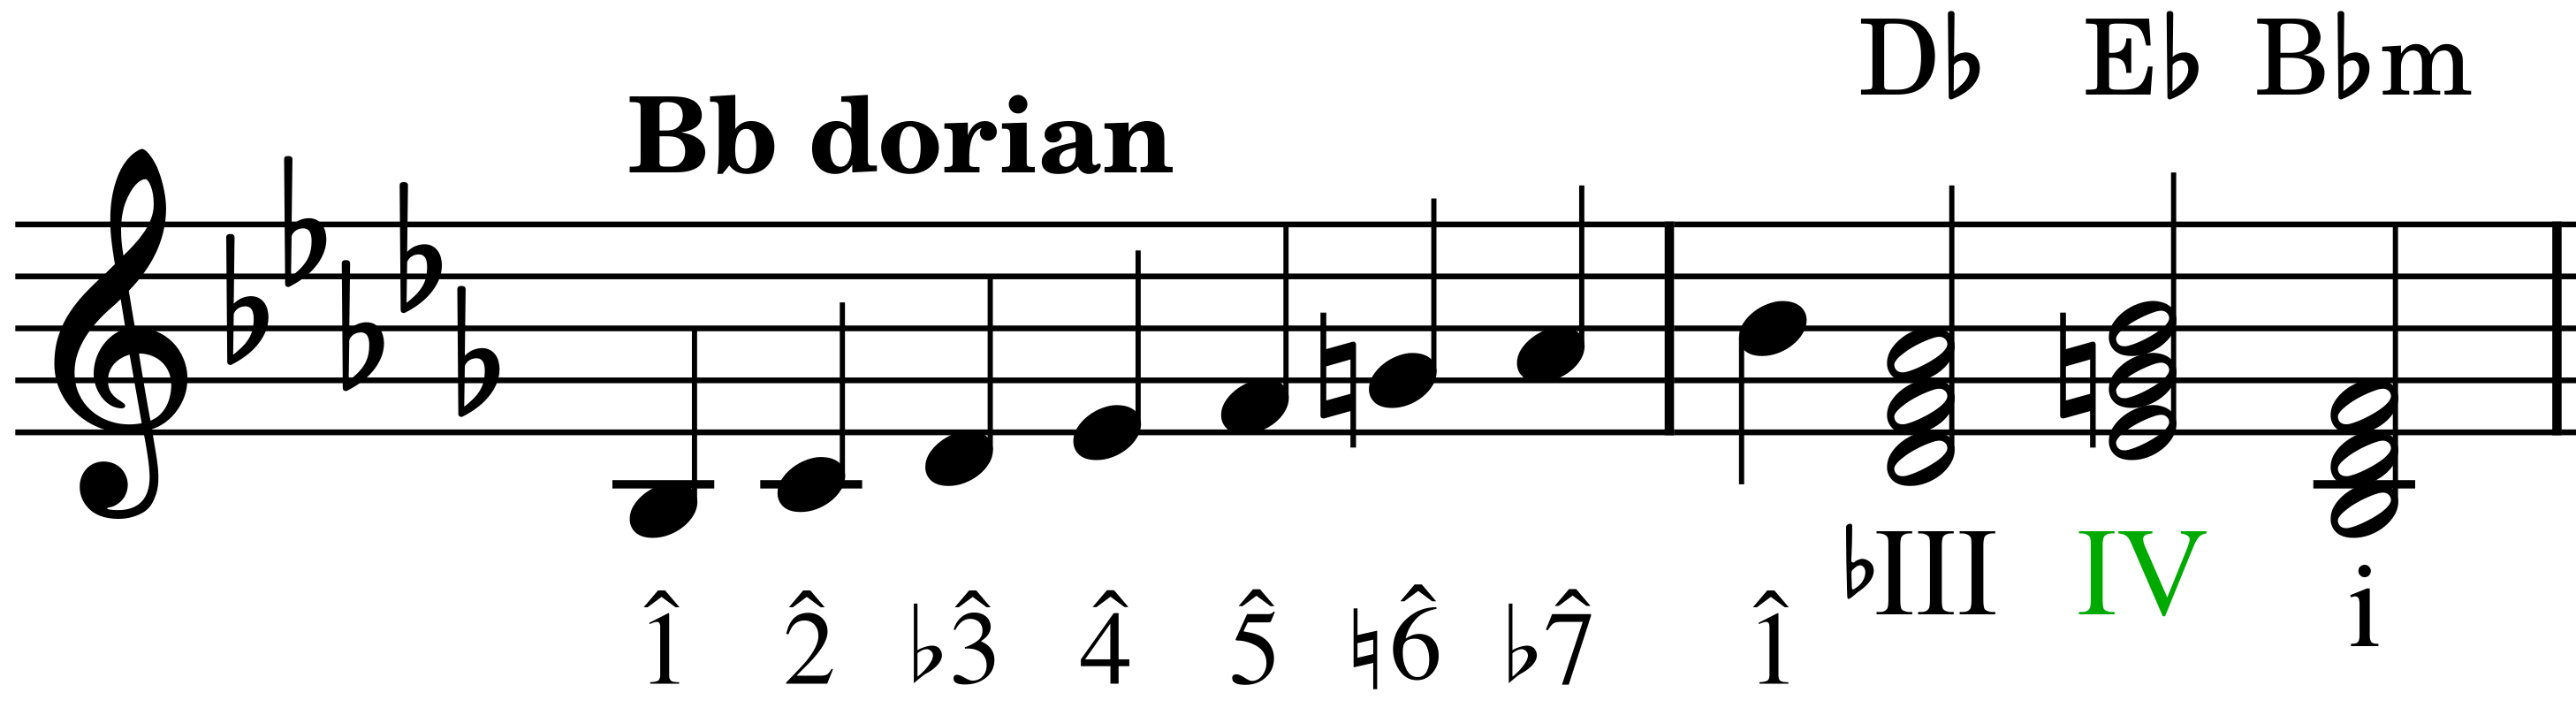
\includegraphics[width=\linewidth]{dorianScale.png}
    \caption{ドリアン音階}
    \label{fig:dorianScale}
\end{figure}
そしてその次にU.N.オーエンのサビを決定的に明るくする和音が一つ入ります。サビ４和音目の\wc{Eb/G\na}では、音階通りのG\fl の音ではなく、音階から外れたG\na の音が用いられております。このG\na は通常の短音階（\autoref{fig:minorScale}）とは別の、ドリアンスケールと呼ばれる明るく勇敢な音階（\autoref{fig:dorianScale}）をイメージさせます。ここで楽曲が一気に明転するということです。もし仮にここで短音階から逸脱しなかった場合の譜例を\autoref{fig:aeolianChorus}に載せました。対応する音声を耳で聴いてみると、原曲と異なって薄暗い印象を与えることがわかります。
\begin{figure}[h]
    \centering
    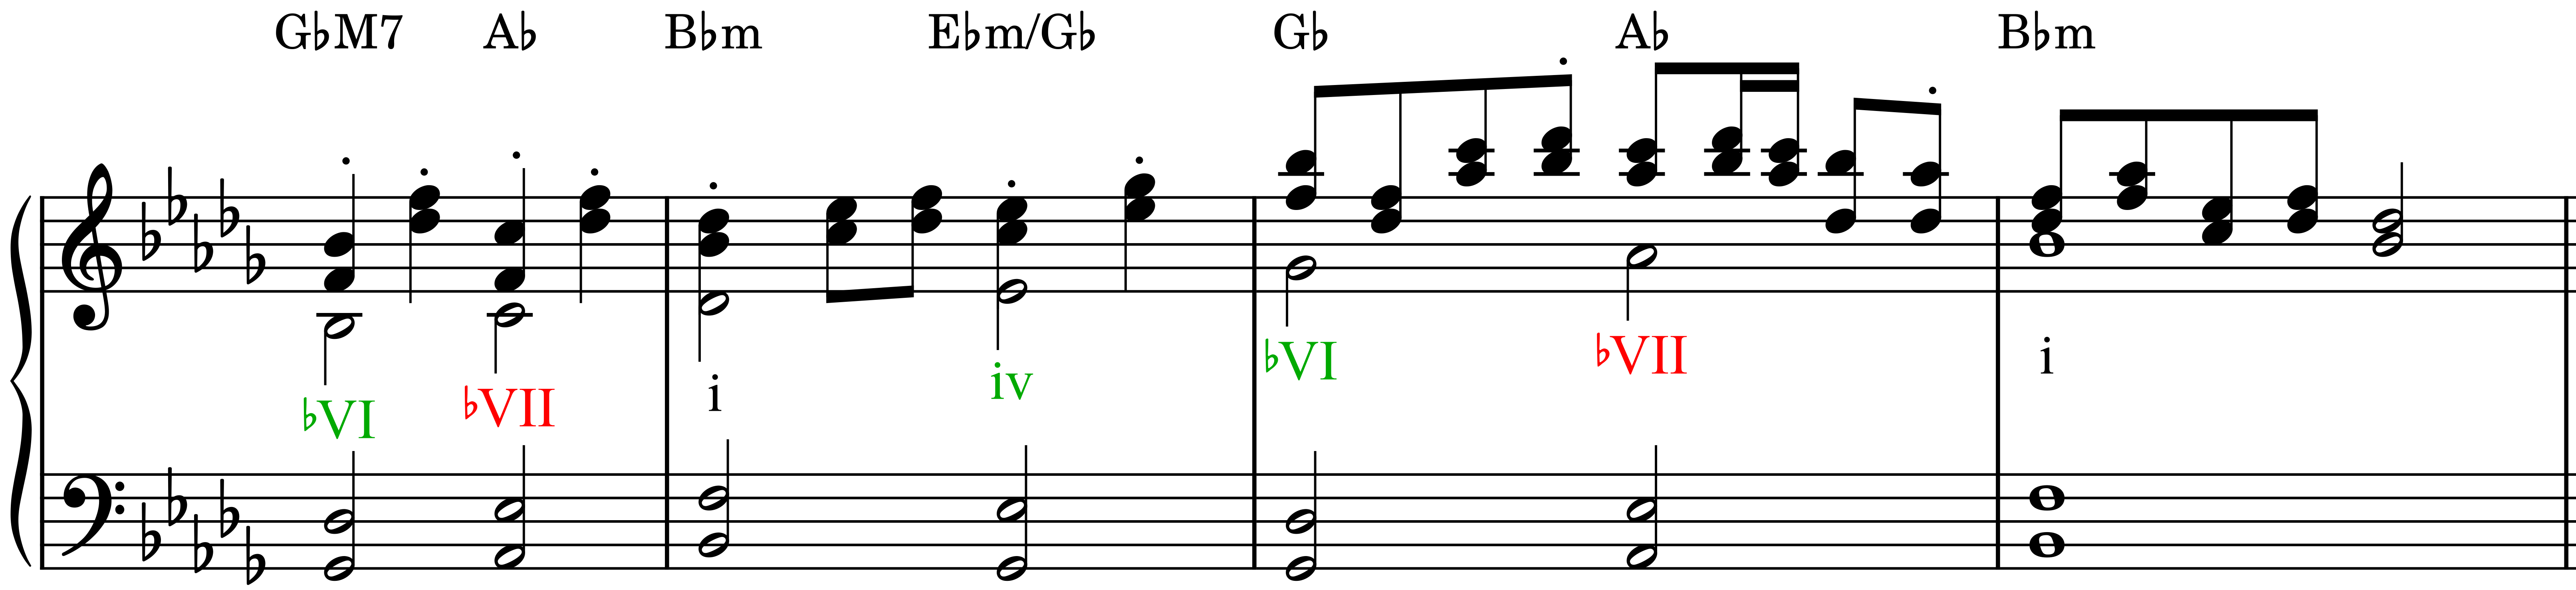
\includegraphics[width=\linewidth]{aeolianChorus.png}
    \caption{仮にサビが音階に忠実な場合}
    \label{fig:aeolianChorus}
\end{figure}
\subsection{2026版についての追記}
紅魔郷New Classicで新しくなったU.N.オーエンでは「希望と未来へと動き出す感情」が少しだけ追加されていると言われています。これについても譜面を見ながら確認してみましょう。\par
2002版と2026版の違いは主に全体のキー設定、１サビの最終和音、及びパワーアップした２サビです。前節で論じたように楽曲の「明るさ」を担うサビが2026版で延長され、新しい対旋律を以て展開されることによって「希望」および「未来へと動き出す感情」が追加されていると解釈することができます。\par
\begin{figure}[h]
    \centering
    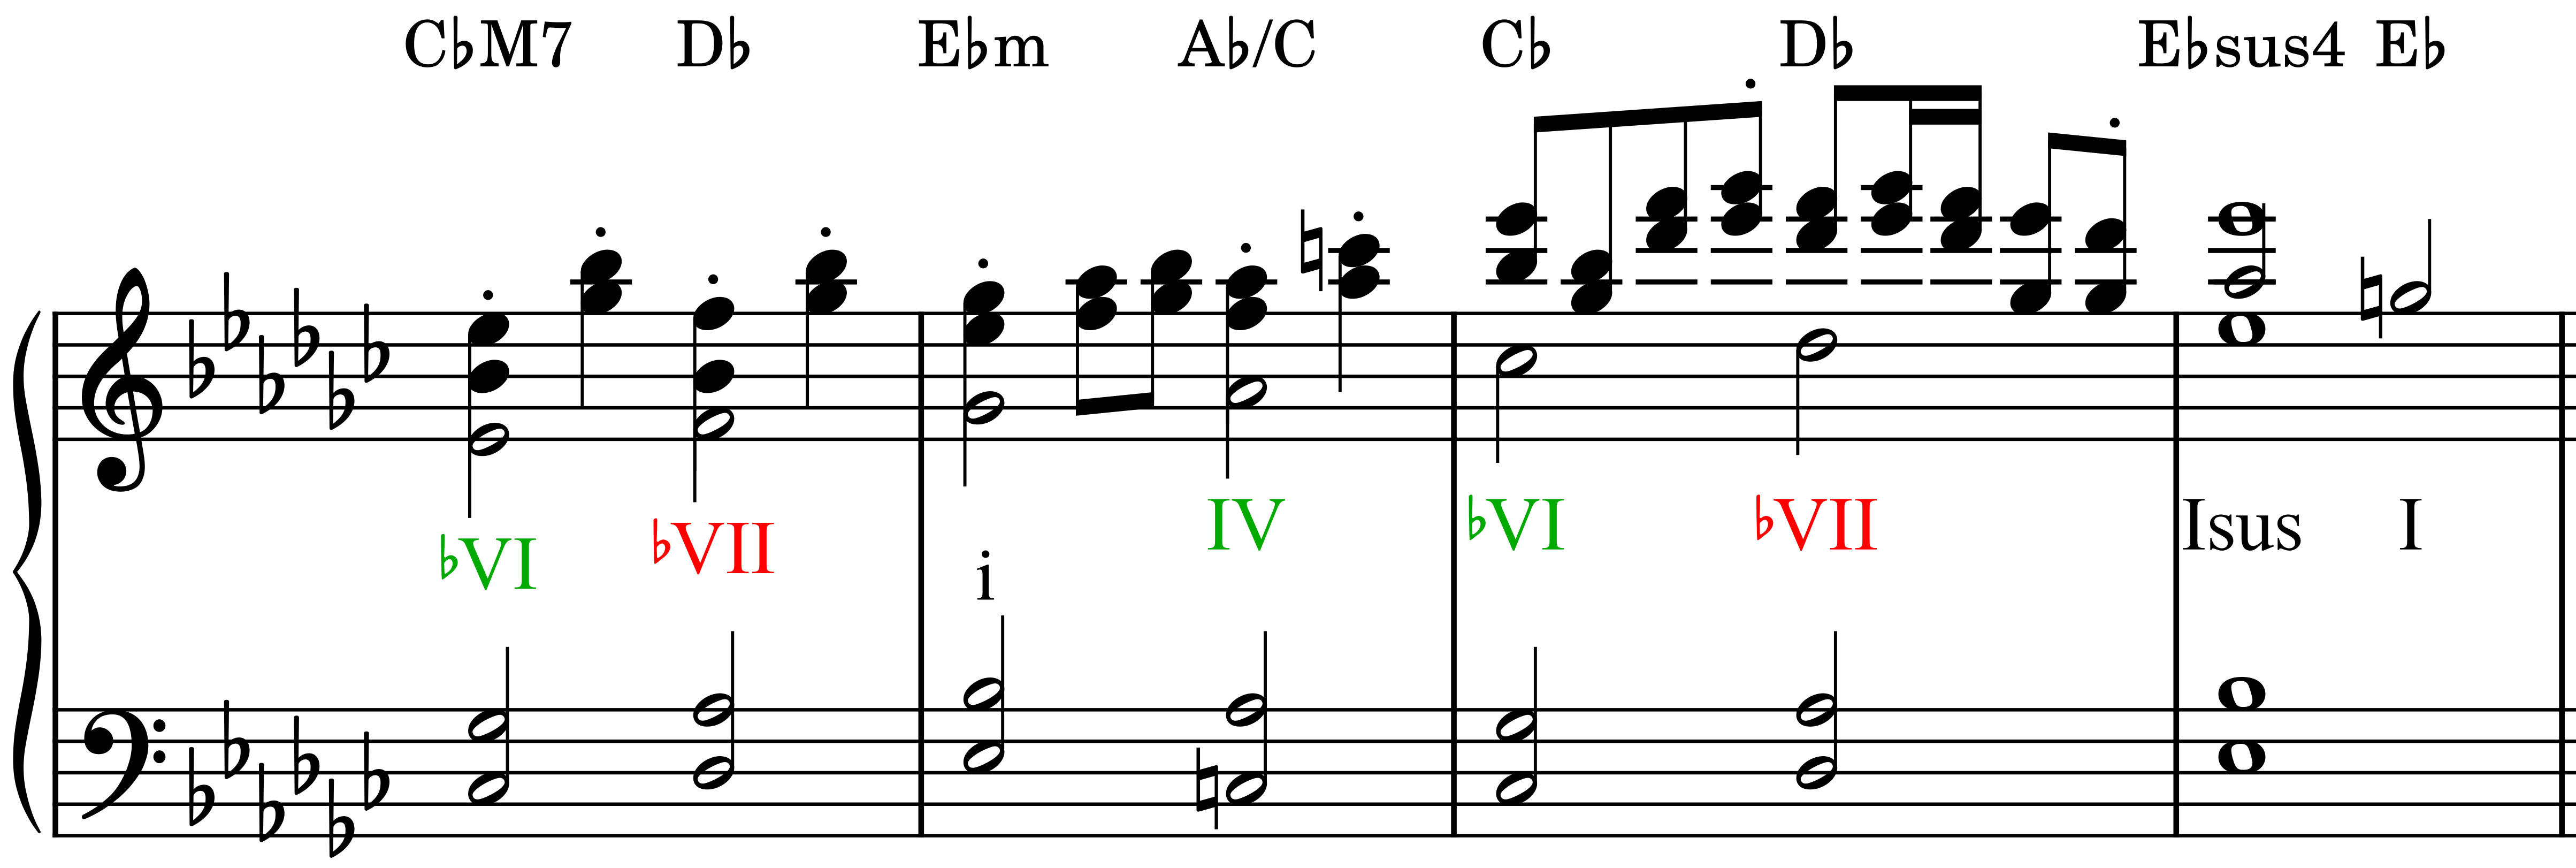
\includegraphics[width=\linewidth]{chorus2026.png}
    \caption{サビ（2026）}
    \label{fig:chorus2026}
\end{figure}
しかし、２サビの変更はそれだけではなく、もう一つ鍵となる和音変更があります。\autoref{fig:chorus2026}の四小節目は、2002版のようにシンプルに終わるのではなく、\wc{Ebsus4}を挟んで\wc{Eb}で終わります。この\wc{Eb}は短音階ではなく長音階で存在する和音で、その使用により楽曲がこの一小節の間だけ一時的に短調から長調へと転じます。これは2002版には無かった更なる「明るさ」で、新たなる希望を示唆すると言えるでしょう。
\subsection{「亡き王女の為のセプテット」との関連性}
最後に、\autoref{sec:chorus}で確認した明るい４和音目について、さらなる解釈の可能性を紹介していきます：実は、上記の明るい和音は「亡き王女のためのセプテット」でも登場します。\par
\begin{figure}[h]
    \centering
    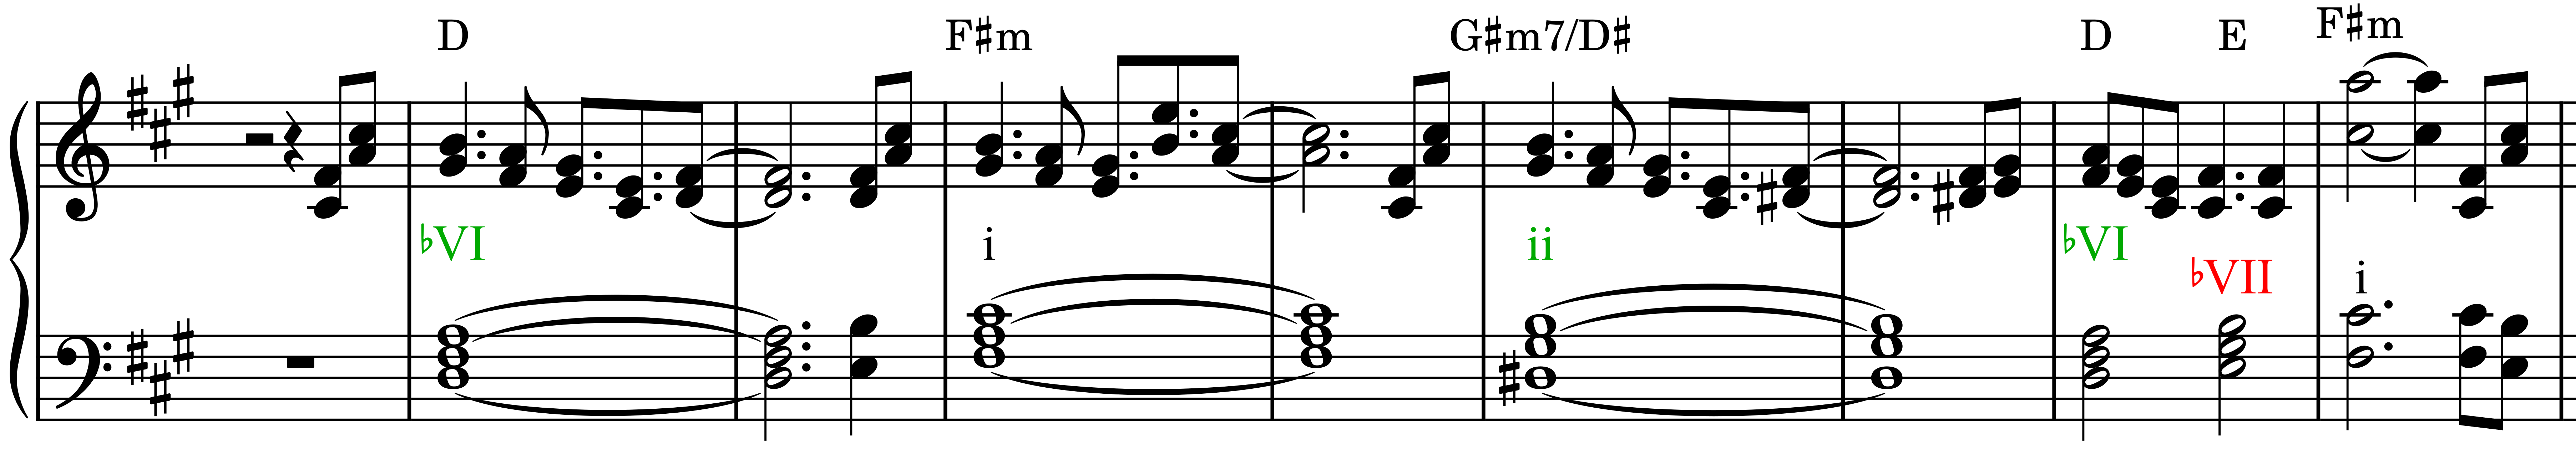
\includegraphics[width=\linewidth]{septetteChorus.png}
    \caption{セプテット（2002）のサビ}
    \label{fig:septetteChorus}
\end{figure}
セプテットの３和音目である\wc{G#m7/D#}は\autoref{sec:chorus}で紹介したドリアンスケール的逸脱音を含み、U.N.オーエンの\wc{Eb/G\na}と本質的にほぼ同じサウンドを持ちます。両者のキーを合わせて比較してみるとわかりやすいでしょう（\autoref{fig:vampireComparison}）。相似点はここだけにとどまらず、\wc{Eb/G\na}の一つ前の和音も同一であるうえ、図中に紫色でマークしたベースラインの動き（\fl\sd{6} \fl\sd{7} \sd{1} \na\sd{6}）も一致します。ここにスカーレット姉妹の設定的な繋がりを見出すことは不可能ではないでしょう。\par
尤も、楽曲中でのドリアンスケールの使用自体はこの二つの曲に限られたものでもなく、他の曲\footnote{ネクロファンタジア、少女が見た日本の原風景、廃獄ララバイ、どうせなら命を賭けて謎を解け　をはじめとして}でもふんだんに使われており、セプテットの中でさえもAメロや間奏でも用いられているので、このようなサウンドが偶然ZUN氏の好みの範疇にあっただけで、スカーレット姉妹の曲で似た和音を用いたことにそれ以上の意図がなかったことも可能です。とはいえ、「ラクトガール ～ 少女密室」（2026）で「レミリアっぽさ」を追加するために\cite{EoSDNC}セプテットからドリアンスケール的フレーズを引用したことが最近注目を浴びているので、実際のところはわからないでしょう。
\begin{figure}[h]
    \centering
    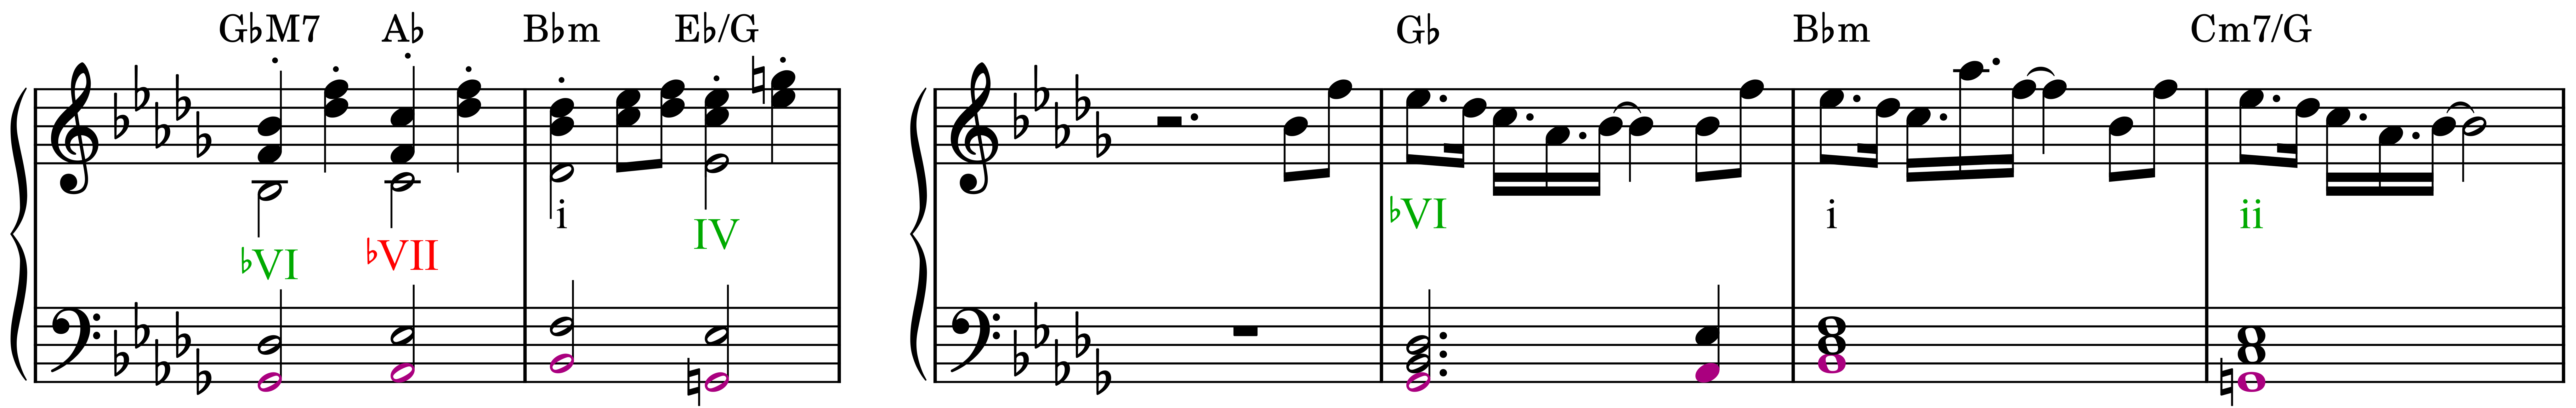
\includegraphics[width=\linewidth]{vampireComparison.png}
    \caption{スカーレット姉妹のサビの比較。セプテットはリズムを速め、キーをU.N.オーエンに合わせた。}
    \label{fig:vampireComparison}
\end{figure}
\subsection{まとめ}
本稿では、「U.N.オーエンは彼女なのか？」を分析し、当楽曲が狂気の音楽として受容されてきた音楽的な理由を説明しました：イントロでは摑みづらい拍子が聴者のリズム感覚を狂わせる中で不可解なシンセサウンドによる不協和音が鳴り響き、Aメロでは方向性の無いメロディー・コード進行が聴者の方向感覚を奪います。そしてサビが終われば遠隔調へ転調し、間もない間に再び主調に戻ります。\par
それに対してサビはわかりやすいコード進行と、短音階から逸脱した明るい和音の借用によって一筋の光を垣間見せます。続けて2026版について見ていき、そのサビの延長・展開や、一時的に長調を示唆する明るい和音改変が「希望」や「未来へと動き出す感情」を反映していると論じました。\par
最後に、U.N.オーエンのサビ４和音目として登場した明るい和音が「亡き王女の為のセプテット」のサビの３和音目でも登場することを示し、スカーレット姉妹のキャラクター表現としての更なる解釈の可能性を提示しました。
\section{付録}
\setcounter{figure}{0}
\renewcommand{\thefigure}{\roman{figure}}
\renewcommand{\thetable}{\roman{table}}
\subsection{楽譜の読み方}
別の合同誌のために書いた注釈のようなものですが、きっと役立つこともあると思ったので、再掲してみます。まえがきのQRからどうぞ！
\subsection{音楽理論のいろは}
頁数の関係でDLコンテンツに動かしました！まえがきのQRからアクセスできます。
\subsection{本稿における表記法と思想}
本稿で使用する表記とコードの解釈について追記します。東方は短調で書かれることが多く、臨時記号も多用するので、それに適応するために短調としてコードを表記していき、臨時記号およびコードの質を明記していきます。\par
また、スケール度数とコードルートに対する度数を区別するために前者をアクセント付きの数字で表記します（\autoref{fig:appendixScales}）。\par
\begin{itemize}
    \item  長音階に関しては \sd{1} \sd{2} \sd{3} \sd{4} \sd{5} \sd{6} \sd{7} と表記
    \item 自然短音階は \sd{1} \sd{2} \fl \sd{3} \sd{4} \sd{5} \fl \sd{6} \fl \sd{7} と表記
    \item その上で、臨時記号をその都度用いる（例: 和声短音階は \sd{1} \sd{2} \fl \sd{3} \sd{4} \sd{5} \fl \sd{6} \na \sd{7} ）
\end{itemize}



コードの質を明記する一貫で、メジャーコードとマイナーコードのローマ数字表記を区別します（\autoref{fig:appendixDiatonicChords}）。
\begin{itemize}
    \item メジャーコードは大文字
    \item マイナーコードは小文字
    \item コードエクステは重要であると判断した場合に表記
\end{itemize}
続いてダイアトニックコードの役割について以下のようにカテゴライズします（\autoref{tab:appendixDiatonicFunctions}）。
\begin{itemize}
    \item 長調
    \begin{itemize}
        \item \writechord{I}, \writechord{iii}, \writechord{vi}はトニック役  
        \item \writechord{V}, \writechord{viio}はドミナント役
        \item \writechord{ii}, \writechord{IV}はプレドミナント役   
    \end{itemize}
    \item 短調
    \begin{itemize}
        \item \writechord{i}, \writechord{bIII}, \writechord{vi}はトニック役  
        \item \writechord{v}, \writechord{bVII}はドミナント役
        \item \writechord{iio}, \writechord{iv}, \writechord{bVI}はプレドミナント役   
    \end{itemize}
\end{itemize}
さらに、今回の寄稿の譜例では従来の機能を持たない和音を青色で表記しております。
\begin{figure}[h]
    \centering
    \begin{subfigure}{0.4\textwidth}
        \centering
        
\includegraphics[width=\linewidth]{appendix/major scale.png}
        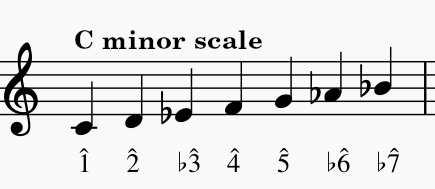
\includegraphics[width=\linewidth]{appendix/minor scale.png}
        \caption{長音階、短音階}
        \label{fig:appendixScales}
    \end{subfigure}
    \begin{subfigure}{0.4\textwidth}
        \centering
        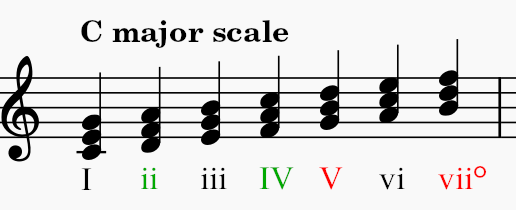
\includegraphics[width=\linewidth]{appendix/major scale chords.png}
        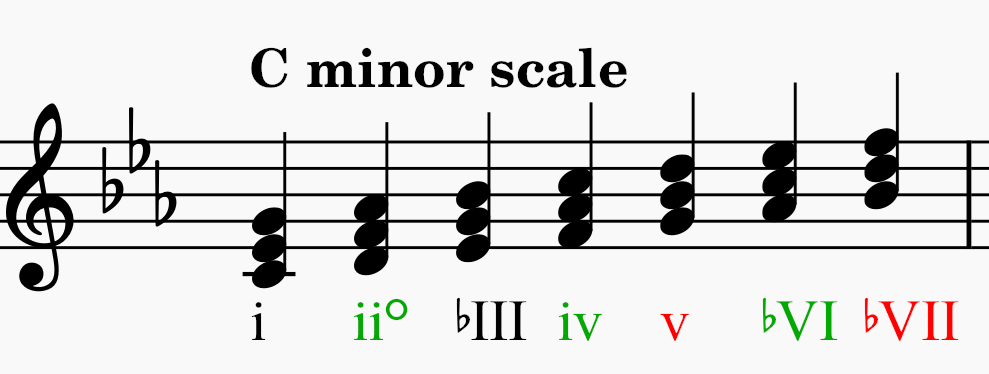
\includegraphics[width=\linewidth]{appendix/minor scale chords.png}
        \caption{長音階、短音階のダイアトニックコード}
        \label{fig:appendixDiatonicChords}  
    \end{subfigure}
    \caption{本稿での表記}
    \label{fig:appendixNotation}
\end{figure}

\begin{table}
    \caption{コードの役割}
    \begin{adjustbox}{max width=\linewidth}
    \begin{tabular}{|c|c|c|c|}\hline
        調 & トニック & \textcolor{BrickRed}{ドミナント} & \textcolor{ForestGreen}{プレドミナント} \\\hline
        長調 & \makecell{\writechord{I} \\ \wc{iii} \\ \wc{vi}} & \makecell{\wc{V} \\ \writechord{viio}} & \makecell{\wc{IV} \\ \wc{ii}} \\
        短調 & \makecell{\writechord{i} \\ \wc{bIII}} & \makecell{\wc{v} \\ \writechord{bVII}} & \makecell{\wc{iv} \\ \writechord{bVI} \\ \wc{iio}} \\ \hline
    \end{tabular}
    \end{adjustbox}
    \label{tab:appendixDiatonicFunctions}
\end{table}

\printbibliography[title=参考文献]

\end{document}
